	\chapter{Système de propulsion}

	Le principe fondamental de déplacement de l'aéroglisseur est basé 
	sur la rotation d'une hélice, qui génèrera le flux d'air nécessaire
	au déplacement de l'aéroglisseur. La mise en rotation de cette hélice
	sera réalisée grâce à un moteur DC \textit{brushless}. 
			
	Dans cette partie, nous développerons dans un premier temps les 
	généralités autour des moteurs DC brushless. Dans un second et 
	troisième temps, nous aborderons les aspects de conception d'un 
	onduleur et de contrôle du moteur avec une méthode ne faisant appel
	à aucun capteur basée sur la lecture du retour de force 
	électromécanique. Une quatrième partie présentera la mise en oeuvre
	d'une simulation \texttt{PSIM} du système et une cinquième partie 
	se concentrera sur les aspects de réalisation d'un PCB de contrôle
	du moteur \textit{brushless}.
	
		\vspace{-1em}
			
		\section{Généralités sur le moteur à courant continu \textit{brushless}}
			
		Comme son nom l'indique, et contrairement à la majorité des moteurs
		à courant continu, le \textbf{moteur à courant continu \textit{brushless}} 
		(en anglais \textit{Brushless DC Motor}, abrégé BLDCM par la suite) 
		\textbf{n'utilise pas de balais}. 
		Les moteurs à courant continu standards disposent en effet de bobinages
		sur le rotor et nécessitent donc un \textbf{collecteur} constitué de
		balais pour alimenter ces bobinages. Cependant, ce collecteur est source
		de nombreux désagréments. Cette pièce est soumise à l'usure et réduit
		considérablement la longévité des moteurs à courant continu. 
		De plus, cette pièce assurant la transmission d'énergie électrique vers
		le rotor est sujette à des pertes énergétiques, qu'elles soient 
		mécaniques ou électriques. 
		
		Historiquement, le moteur à courant continu a toujours été populaire
		du fait de la facilité de réglage de la vitesse ou du couple de sortie. 
		Les innovations dans les champs
		de l'électronique de puissance, mais aussi l'apparition progressive
		des microprocesseurs aves des capacités de calcul de plus en plus 
		importantes permettent par la suite une ouverture à de nouvelles 
		possibilités de contrôle des moteurs. 
	
	 	L'absence de balais dans le moteur \textit{brushless} implique
	 	donc une commutation électronique de l'alimentation des enroulements
	 	statoriques. 
	 	L'utilisation d'une telle structure fait que le BLDCM a de nombreux
	 	avantages par rapport aux moteurs DC à balais ou les moteurs à 
	 	induction. Parmi ces avantages, on peut notamment retenir :
	 	
	 	\vspace{0.5em}
		
		\begin{itemize}
			\item[$\bullet$] des caractéristiques couple / vitesse améliorées ;
			\item[$\bullet$] une prolongation de la durée de vie du moteur ;
			\item[$\bullet$] des fonctionnements moins bruyants ;
			\item[$\bullet$] des performances en vitesse augmentées.
		\end{itemize}
		
		\vspace{0.5em}
			
		De plus, le rapport couple délivré / encombrement moteur 
		est amélioré, ce qui rend le BLDCM très utile dans des 
		applications où l'espace et le poids sont des critères 
		cruciaux \cite{AN885}, comme dans le cas de notre aéroglisseur.
			
			\subsection{Structure du moteur brushless}
				
			Un moteur brushless est structuré à partir d'un aimant permanent
			au rotor et de pôles bobinés au stator. L'énergie électrique est
			convertie en énergie mécanique par le biais des forces d'attraction
			magnétique entre l'aimant permanent du rotor et le champ tournant
			induit par les pôles bobinés du stator. 
			La \textsc{Figure \ref{struct_bldcm}} présente une illustration 
			simplifiée de la construction d'un BLDCM. 
				 
			\begin{figure}
				\begin{center}
				 	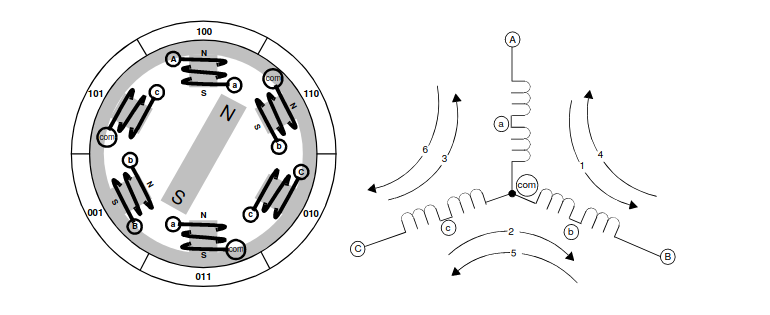
\includegraphics[scale=0.7]{../Illus/struct_bldcm.png}
				\end{center}
				\caption{Diagramme simplifié de la structure d'un BLDCM (\textit{Source :} \cite{AN857})}
				\label{struct_bldcm}
			\end{figure}
				 
			L'exemple de structure présenté ici montre trois circuits 
			électromagnétiques connectés à un point commun (couplage étoile). 
			Chacun des circuits est divisé en deux parties qui seront bobinées
			sur des dents de la machine diamétralement opposées. 
			Cette structure permet alors à l'aimant permanent au rotor de se
			déplacer au milieu de champs magnétiques induits. 
			Nous avons modélisé le BLDCM en utilisant le logiciel \textit{FEMM}
			pour donner une idée plus concrète de son fonctionnement en rotation. 
				 
			\subsection{Modélisation}
				 
			La modélisation sous le logiciel \textit{FEMM} permet notamment d'observer
			les modifications du champ magnétique dans le cas d'un changement
			séquentiel de l'alimentation des enroulements statoriques.
				 
			Une \href{https://www.youtube.com/watch?v=pMH3krwI\_W0}{\textcolor{blue}{vidéo}}, 
			réalisée par nos soins lors d'un électif les années
			précédentes avec M. Flieller, permet de mieux illuster l'effet
			de cette séquence de commutation sur la mise en mouvement d'un
			moteur \textit{brushless}. La modélisation présentée montre
			notamment un fonctionnement pas-à-pas du moteur.
						 
	\newpage
	
	\section{Onduleur triphasé}
	\label{onduleur}		%Tu peux la mettre où tu veux juste la où tu présente l'onduleur
							%Du coup je te l'ai mis là
							
	La plupart des BLDCM ont une structure triphasée avec un 
	couplage étoile, et c'est notamment le cas du moteur que 
	nous allons utiliser dans ce projet. 
	Un tel moteur est alors piloté en alimentant deux phases 
	en même temps. Afin d'entrer en rotation, les trois phases
	du moteur devront être alimentées successivement suivant 
	une séquence précise comme le montre la 
	\textsc{Figure \ref{waveforms}}.
	Afin de mettre en oeuvre cette séquence, il est nécessaire
	de passer par un onduleur triphasé.
	
		\subsection{Structure d'un onduleur triphasé}
		
		Le principe de l'onduleur triphasé va être de pouvoir
		alimenter chaque phase à un niveau haut, bas ou flottant
		suivant le moment précis auquel on se trouve dans la 
		séquence de commutation.
		
		\begin{figure}[h]
			\begin{center}
				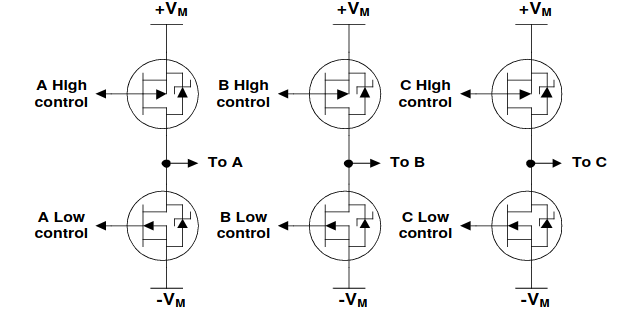
\includegraphics[scale=0.8]{../Illus/bridge_princ.png}
			\end{center}
			\caption{Structure de principe d'un onduleur triphasé}
			\label{bridge_princ}
		\end{figure}
		
		\newpage
	
		\subsection{Séquence de commutation}
		
		La \textsc{Figure \ref{waveforms}} montre un exemple
		des formes d'ondes de capteurs à effets Hall et de
		retour de force électromotrice sur un moteur \textit{brushless}.
		
		\begin{figure}[h]
			\begin{center}
				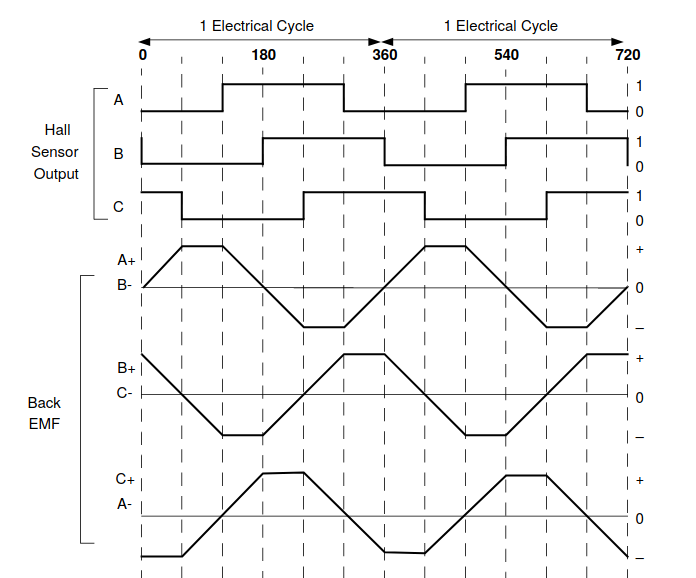
\includegraphics[scale=0.7]{../Illus/waveforms.png}
			\end{center}
			\caption{Formes d'ondes des capteurs à effet Hall et des forces électromotrices sur
			deux tours électriques}
			\label{waveforms}
		\end{figure}
		
		Chaque 60 degrès de la rotation électrique, un capteur à effet Hall
		change d'état. En prenant en compte cette observation, on en déduit
		qu'il y a six étapes pour faire un tour électrique complet.
		
		Il faut également garder en tête qu'un tour électrique
		ne correpond par forcément à un tour mécanique. En effet, le
		nombre de cycles électriques pour compléter un tour mécanique
		est déterminé par le nombre de paires de pôles du moteur en
		suivant la relation (\ref{speed_pole}).
		
		\begin{equation}
		\Omega=\frac{\omega}{p}
		\label{speed_pole}
		\end{equation}
		
		où $\Omega$ est la vitesse angulaire mécanique
		et $\omega$ est la vitesse angulaire électrique.
	
	\newpage
	
	\section{Retour de force électromotrice}
	
	Il est important de remarquer que le moteur \textit{brushless}
	utilisé dans notre conception ne possède pas de capteurs à 
	effet Hall. Cet avantage, notamment en matière d'encombrement
	et de poids, pose au contraire une problématique lorsqu'il
	s'agit de localiser le rotor en vue d'appliquer une séquence
	de commutation électronique adéquate. Une solution pour
	pallier à ce problème est de se baser sur le retour de force 
	électromotrice des phases. Cette méthode va être présentée
	dans cette section.
	
		\vspace{-1em}
	
		\subsection{Théorie magnétique}
		
		Lorsqu'un moteur \textit{brushless} tourne, chaque enroulement 
		statorique génère une tension dite \textbf{force électromotrice},
		opposée à l'alimentation des enroulements suivant la 
		\textbf{loi de Lenz}.
	
		Cette force électromotrice dépend de trois facteurs principaux
		qui sont :
		
		\begin{itemize}
			\item[$\bullet$] la \textbf{vitesse angulaire} du rotor ;
			\item[$\bullet$] le \textbf{champ magnétique} généré par les aimants du rotor ;
			\item[$\bullet$] le \textbf{nombre de tours} des enroulements statoriques.
		\end{itemize}
		
		L'équation (\ref{bemf_law}) donne l'expression de proportionnalité
		entre la valeur de la force électromotrice et la valeur des 
		facteurs cités ci-dessus.
		
		\begin{equation}
			E\quad\alpha\quad
			NlrB\omega
			\label{bemf_law}
		\end{equation}
		
		\begin{itemize}
			\item[$\bullet$] $N$ le nombre de tours d'enroullement par phase ;
			\item[$\bullet$] $l$ la longueur du rotor ;
			\item[$\bullet$] $r$ le rayon interne du rotor ;
			\item[$\bullet$] $B$ la densité magnétique de champ dans le rotor ;
 			\item[$\bullet$] $\omega$ la vitesse angulaire du moteur.
		\end{itemize}
		
		\vspace{-1em}
		
		\subsection{Implémentation pratique}
		
		Pratiquement, l'objectif est de localiser le passage en zéro de
		la force électromotrice généré par une phase comme montré
		en \textsc{Figure \ref{waveforms}}. Pour cela, on se base sur
		la relation (\ref{bemf_prat}) donnant la force électromotrice $E_A$ d'une 
		phase (la phase A, prise ici en exemple) en fonction des trois 
		tensions simples $V_A$, $V_B$ et $V_C$ mesurées aux bornes du moteur.
		
		\begin{equation}
		E_A =\frac{2}{3}\cdot V_A - \frac{1}{3}\cdot V_B - \frac{1}{3}\cdot V_C
 		\label{bemf_prat}
		\end{equation}
		
		Il suffit alors d'implémenter un comparateur en pondérant via
		des ponts diviseurs de tension les différentes tensions simples
		afin d'obtenir la détection souhaitée. La 
		\textsc{Figure \ref{bemf_comp}}
		montre un circuit permettant de réaliser cette fonction.
		
		\begin{figure}[h]
			\begin{center}
				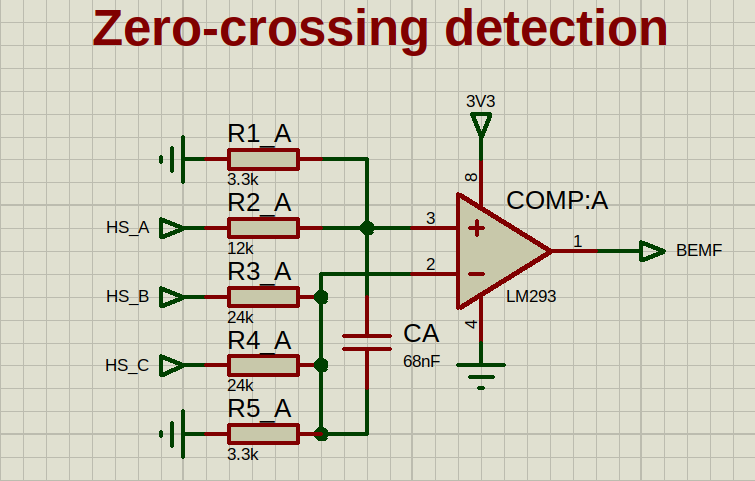
\includegraphics[scale=0.25]{../Illus/bemf_comp.png}
			\end{center}
			\vspace{-1.5em}
			\caption{Circuit de détection du passage en zéro d'une force
			électromotrice}
			\label{bemf_comp}
		\end{figure}
		
	\newpage
				 
	\section{Modélisation électrique du système de propulsion}
			
	Le système complet de propulsion va être modélisé sous le logiciel \textsc{PSIM}.
	La simulation comprendra notamment l'onduleur triphasé, le moteur \textit{brushless} 
	de propulsion ainsi qu'une modélisation mathématique de l'hélice.
	
		\vspace{-1em}
			
		\subsection{Modélisation de l'onduleur triphasé} 
		
		L'onduleur triphasé va être représenté sous \textsc{PSIM} par
		les six transistors MOSFETs comme représentés en 
		\textsc{Figure \ref{bridge_struct_psim}}.
		
		\begin{figure}[h]
			\begin{center}
				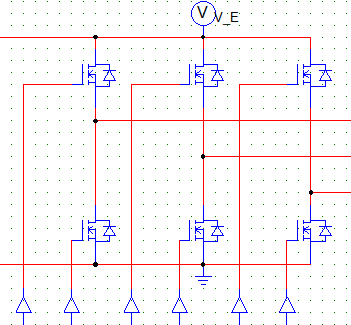
\includegraphics[scale=0.5]{../Illus/bridge_struct_psim.png}
			\end{center}
			\vspace{-1em}
			\caption{Structure de l'onduleur triphasé sous \textsc{PSIM}}
			\label{bridge_struct_psim}
		\end{figure}
		
		Nous devrons notamment saisir les paramètres caractéristiques
		de chaque MOSFET afin de simuler au mieux le fonctionnement
		des MOSFETs canal N \texttt{BSC0902NS} utilisés.
		La liste des différents paramètres d'un modèle de MOSFET sous 
		\textsc{PSIM} est montrée en \textsc{Figure \ref{mosfet_model_psim}}.
		
		\begin{figure}[h]
			\begin{center}
				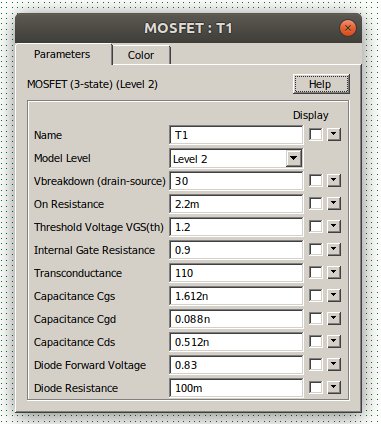
\includegraphics[scale=0.65]{../Illus/mosfet_model_psim.png}
			\end{center}
			\vspace{-1em}
			\caption{Paramètres d'un modèle de MOSFET canal N sous \textsc{PSIM}}
			\label{mosfet_model_psim}
		\end{figure}			
				
		\subsection{Modélisation du moteur DC brushless}
			
		Un élément de la bibliothèque de PSIM permet de modéliser
		le moteur DC \textit{brushless} du système de propulsion.
		
		La \textsc{Figure \ref{psim_model_bldcm}} montre la symbolisation
		de cet élément ainsi que les différentes caractéristiques qui seront
		à saisir afin d'obtenir un modèle le plus fidèle possible du
		moteur \textbf{NM Prodrive 3350 1100kV} réel.
		
		\begin{figure}[h]
			\begin{center}
				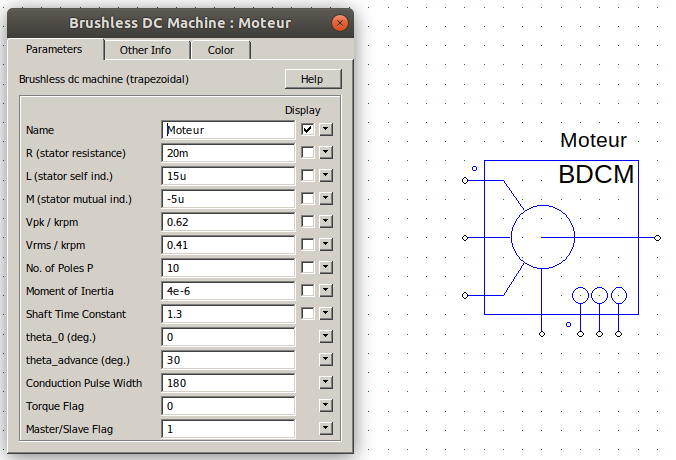
\includegraphics[scale=0.55]{../Illus/psim_model_bldcm.png}
			\end{center}
			\caption{Élément \textit{PSIM} modélisant le moteur DC 
			\textit{brushless} de propulsion}
			\label{psim_model_bldcm}
		\end{figure}
		
			\subsubsection{Valeurs du modèle de phase équivalente}
			
			Nous n'avons pas eu le temps de réaliser une caractérisation
			complète du moteur sur son banc avant l'épisode du confinement.
			Nous avons donc repris pour les valeurs du modèle de phase
			équivalente les valeurs issues du modèle donné par les
			professeurs. Nous avons notamment retenu pour la résistance
			de phase $R$, l'inductance propre de phase $L$ et l'inductance
			mutuelle de phase $M$ respectivement les valeurs 
			(\ref{values_phase}).
			
			\begin{equation}
			R = 20m\Omega
			\quad\quad
			L = 15\mu F
			\quad\quad
			M = -5\mu F
			\label{values_phase}
			\end{equation}
		
			\subsubsection{Nombre de pôles}
			
			Une observation rapide du moteur sur le banc de test
			en début de semestre nous avait permis de déterminer 
			que le moteur \textbf{NM Prodrive 3350 1100kV} possède
			\textbf{10 pôles}, soit $p=5$ paires de pôles.
			
			\subsubsection{Moment d'inertie}
			
			Le moment d'inertie du moteur a été réglé pour la
			simulation à $J=4\cdot 10^{-6}\ kg \cdot m^2$.
			Cette valeur n'a pas de réalité physique par rapport
			au moteur réel, mais permet de réduire les temps de simulation
			pour obtenir des vitesses nominales de fonctionnement.
				
			\subsubsection{Angle d'avance}
					
			C'est un paramètre de simulation très important si l'on veut
			pouvoir accéder à des vitesses de rotation intéressantes pour
			notre système. Afin de mieux présenter ce paramètre et de 
			comprendre son sens physique, nous allons proposer ici une 
			analogie avec l'avance à l'allumage d'un moteur thermique.
			
			\textit{Un moteur thermique est constitué de pistons et de 
			cylindres et dispose d'un système d'allumage permettant de générer
			une étincelle dans les cylindres, provoquant la poussée du
			piston et donc l'entrainement de l'arbre central du système.}
					
			\textit{Lorsque l'avance est nulle, alors l'étincelle arrivera juste
			au moment où le piston est en haut du cylindre. Le front de flamme
			aidera juste à pousser le piston dans sa redescente. Cette séquence
			est fonctionnelle mais n'est pas optimisée.}
			
			\textit{Si une avance est générée, alors l'éticelle commencera à emflammer 
			le mélange de carburant un peu avant que le piston atteigne le point 
			mort haut. Le front de flamme est donc déjà bien avancé quand le piston
			arrivera et il recevra ainsi plus de puissance pour redescendre car 
			bénéficiant d'une pression plus forte.}
			
			\textit{En mettant encore plus d'avance, donc en avançant encore plus le moment
			lors duquel l'étincelle est générée le piston va forcer pour finir de 
			monter (entrainé par les autres pistons ou par son inertie) et va 
			finalement "rebondir" sur le mélange deja en grande partie dilaté.
			Il ne faut donc pas aller plus loin car il risque d'y avoir des retours
			ou des claquements dans le cycle de fonctionnement. }

			\textit{Ce temps d'avance dépend de plus de la vitesse de rotation, plus le moteur
			tourne vite et plus il faudra générer un angle d'avance grand.}
			
			Cette analogie est facilement transposable à la structure
			du moteur \textit{brushless}. Il faudra juste se représenter
			l'\textit{étincelle} comme l'alimentation des bobines statoriques
			et le \textit{piston} comme un pôle du rotor.
			
			On comprend donc aisément que l'angle $\Theta$ d'avance
			électrique peut être pertinemment réglé dans la plage
			\begin{equation}
			\Theta\in [0^{\circ},60^{\circ}]
			\end{equation}
			pour obtenir des effets intéressants sur les performances 
			du moteur \textit{brushless}. L'angle d'avance est un 
			paramètre à régler en prenant également en compte le nombre
			de paires de pôles du moteur utilisé.
			
		\vspace{-1em}
			
		\subsection{Modélisation de l'hélice}
				
		L'hélice est également prise en compte dans la simulation avec
		l'utilisation d'un élément \textit{charge mécanique}.
		Les différents paramètres de cet élément sont donnés
		en \textsc{Figure \ref{helice}}.
		
		\begin{figure}[h]
			\begin{center}
				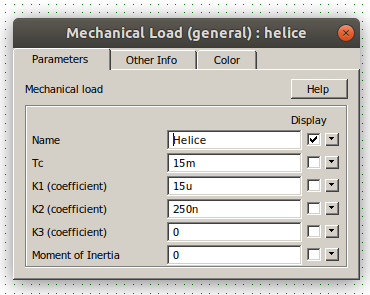
\includegraphics[scale=0.5]{../Illus/helice.png}
			\end{center}
			\vspace{-1em}
			\caption{Paramètres de l'élément \textit{charge mécanique} simulant l'hélice}
			\label{helice}
		\end{figure}
				
		%\subsection{Résultats de simulation}
		
		%Les résultats de simulation...
	
	\newpage		
		
	\section{Réalisation de la carte de l'onduleur}
	
		\subsection{Schéma global de l'onduleur}
		
		La carte de l'onduleur sert de support aux trois bras de
		pont et permet de générer avec le \texttt{DsPIC} les différents
		signaux PWM de contrôle du moteur \textit{brushless}.
		
		L'arrivée d'alimentation sur cette carte se fait avec deux
		connecteurs distincts. Un premier permet d'obtenir la tension
		batterie pour l'alimentation des bras de pont avec un T-BLOCK
		connection vis. L'autre arrivée se fait via un connecteur de 
		nappe 6 points, avec la connection série vers la carte de
		commande permettant de recevoir les ordres de commande du
		moteur ainsi que l'alimentation du microcontrôleur.
		
		La carte dispose également d'un connecteur permettant le
		branchement d'un \texttt{PicKit} afin de programmer le \texttt{DsPIC}.
		
		La \textsc{Figure \ref{bridge_gen_scheme}} présente le schéma
		global de la carte de l'onduleur.
		
		\subsection{Routage de l'onduleur}
		
		Le PCB de l'onduleur peut être considéré comme constitué
		de deux parties distinctes. Une première partie de la carte
		aura son propre plan de masse et permettra de générer les
		signaux de PWM grâce au DsPIC. Cette partie comprend aussi
		le circuit de détection de force électromotrice, qui permettra
		la localisation du rotor à chaque nouveau tour électrique.
		
		Une seconde partie est constituée avec les plans d'alimentation
		des bras de pont ainsi que leurs connecteurs. L'alimentation
		se fait via la couche \texttt{bottom} de la carte tandis que les 
		signaux de PWM et de retour de force électromotrice transitent
		par des pistes sur la couche \texttt{top} du PCB. 
		
		La \textsc{Figure \ref{bridge_gen_routing}} présente le routage
		global de la carte de l'onduleur.
		
		\subsection{Vue 3D de l'onduleur}
		
		En associant chaque modèle 3D au format \texttt{STEP} (\texttt{.stp})
		à chaque composant routé sur la carte, on peut obtenir une vue 3D
		de la carte de l'onduleur. On y remarque notamment le volume des 
		connecteurs bras de pont ainsi que les deux CI utilisés, le \texttt{DsPIC}
		ainsi que le comparateur.

		La \textsc{Figure \ref{bridge_gen_3dview}} présente la vue 3D
		de la carte de l'onduleur.
		
		\newpage
	
		\begin{landscape}
		
		\begin{figure}
			\begin{center}
				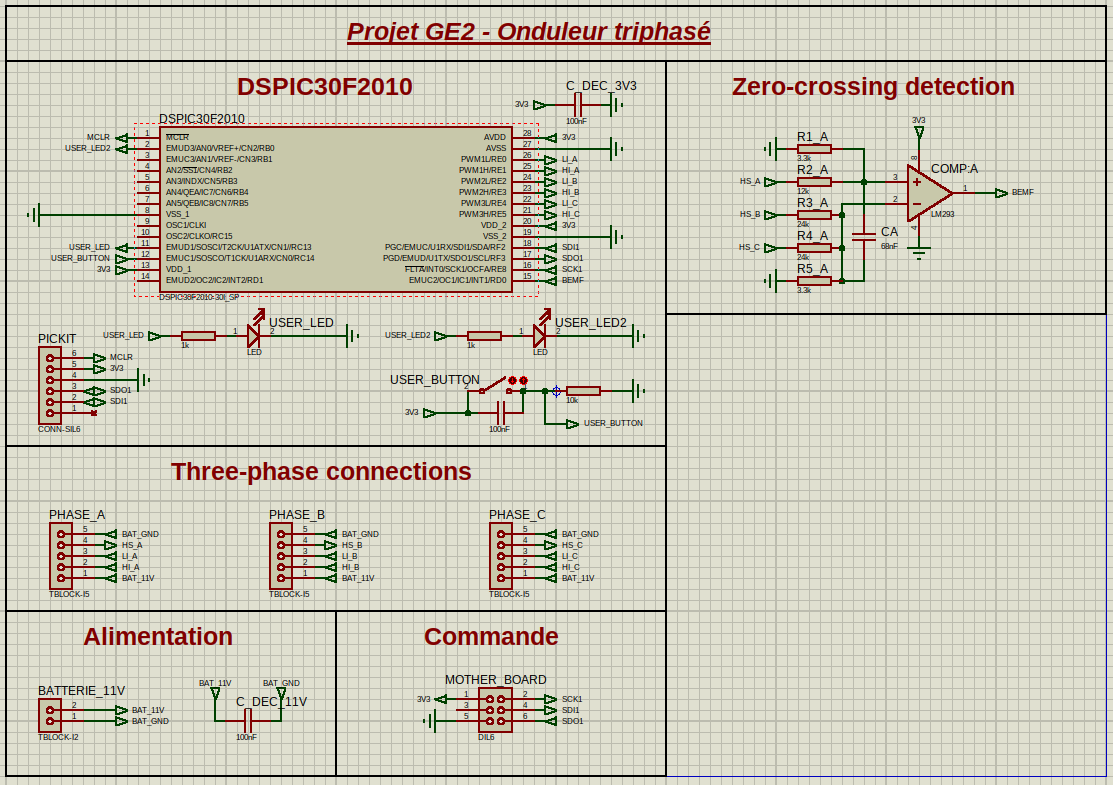
\includegraphics[scale=0.6]{../Illus/bridge_gen_scheme.png}
			\end{center}
			\caption{Schéma global de l'onduleur}
			\label{bridge_gen_scheme}
		\end{figure}
		
		\newpage

		\begin{figure}
			\begin{center}
				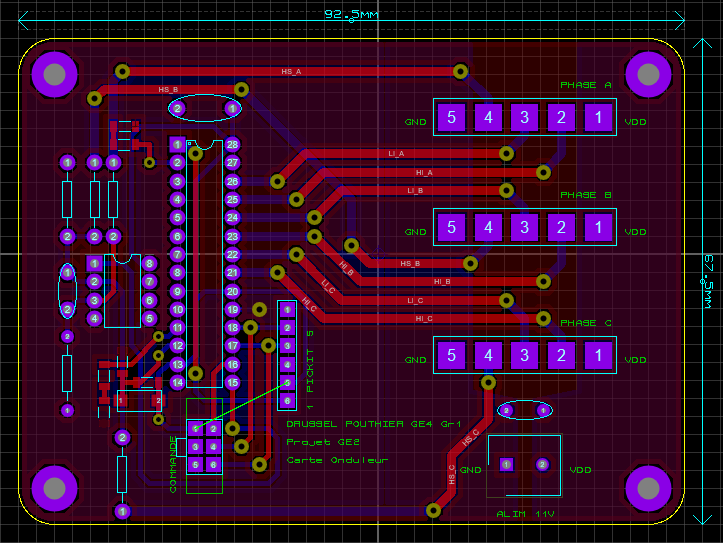
\includegraphics[scale=1.1]{../Illus/bridge_gen_routing.png}
			\end{center}
			\caption{Routage global de la carte onduleur}
			\label{bridge_gen_routing}
		\end{figure}
		
		\newpage
		
		\begin{figure}
			\begin{center}
				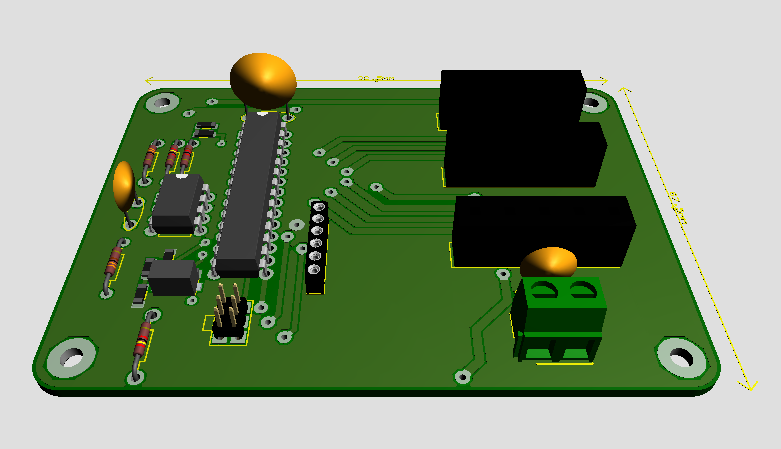
\includegraphics[scale=1.2]{../Illus/bridge_gen_3dview.png}
			\end{center}
			\caption{Vue 3D de la carte onduleur}
			\label{bridge_gen_3dview}
		\end{figure}
		
		\end{landscape}	 
	
		\newpage
		
	\section{Réalisation des cartes bras de pont}
	
		\subsection{Schéma d'un bras de pont}
		
		Le schéma d'un bras de pont est ainsi constitué de deux MOSFETs,
		du driver de demi-pont ainsi que d'un condensateur de découplage de
		l'alimentation.
		
		La \textsc{Figure \ref{phase_gen_scheme}} présente le schéma
		d'une carte bras de pont.
		
		
		\subsection{Routage d'une carte bras de pont}
		
		Afin d'optimiser la surface des cartes bras de pont, il a 
		été retenu de positionner un transistor sur chacune des faces
		des cartes. Cette disposition permet ainsi de respecter les
		contraintes de surfaces d'échange pour les drains des MOSFETs
		tout en limitant la taille globale de carte. Les surfaces
		sont paramétrées avec une distance d'isolement de 10th.
		
		La \textsc{Figure \ref{phase_gen_routing}} présente le routage
		global d'une carte bras de pont.		
		
		\subsection{Vue 3D d'une carte bras de pont}

		La vue 3D de la carte bras de pont prend ici toute son
		importance puisqu'elle permettra de vérifier que le
		volume d'un bras de pont ne vienne pas collapser avec
		le bras de pont voisin. La principale contrainte
		de volume sur ces cartes est notamment la hauteur du
		condensateur de découplage.
		
		La \textsc{Figure \ref{phase_gen_3dview}} présente la vue
		3D d'une carte bras de pont.

		\newpage
		
		\begin{landscape}
		
		\begin{figure}
			\begin{center}
				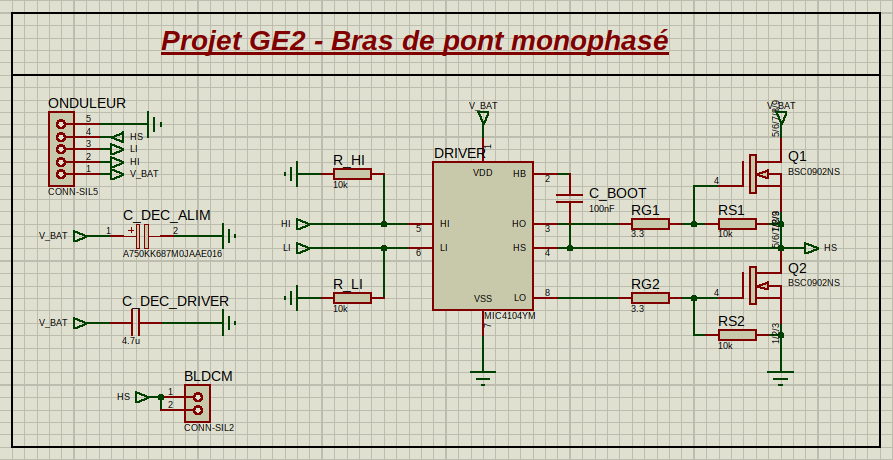
\includegraphics[scale=0.7]{../Illus/phase_gen_scheme.png}
			\end{center}
			\caption{Schéma global d'un bras de pont monophasé}
			\label{phase_gen_scheme}
		\end{figure}
		
		\newpage

		\begin{figure}
			\begin{center}
				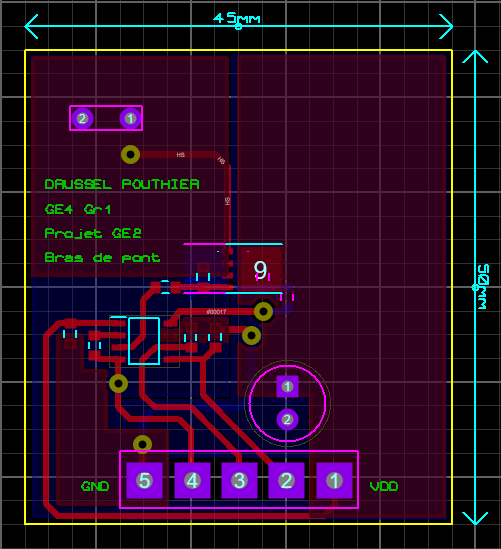
\includegraphics[scale=1]{../Illus/phase_gen_routing.png}
			\end{center}
			\caption{Routage global d'un bras de pont monophasé}
			\label{phase_gen_routing}
		\end{figure}
		
		\newpage
		
		\begin{figure}
			\begin{center}
				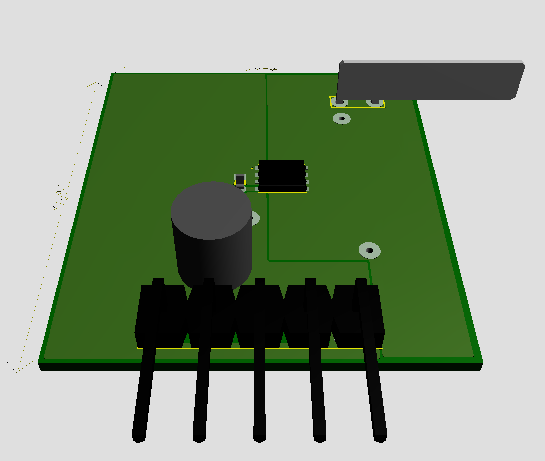
\includegraphics[scale=1.3]{../Illus/phase_gen_3dview.png}
			\end{center}
			\caption{Vue 3D d'un bras de pont monophasé}
			\label{phase_gen_3dview}
		\end{figure}
		
		\end{landscape}	 
		
		\newpage
			
	\section{Conclusions sur le système de propulsion}
	
	Le système de propulsion est un élément central de la conception
	de l'aéroglisseur. Basé sur un moteur de type \textit{brushless}
	entraînant une hélice, il nécessite une conception électronique 
	précise du fait de la commutation électronique requise pour le 
	pilotage du moteur. Il faut également prendre en compte dans la
	conception les valeurs importantes de courant circulant vers le
	moteur et donc adapter le dimensionnement des PCB en fonction.   
	
	La partie suivante va introduire des notions supplémentaires
	sur le contrôle d'un moteur brushless en abordant notamment
	la nature des signaux PWM à générer pour atteindre les
	vitesses de fonctionnement espérées. 
	
\newcommand{\pic}{\texttt{PIC16F1619} }
\newcommand{\dspic}{\texttt{dsPIC30F2010} }